%%%%%%%%%%%%%%%%%%%%%%%%%%%%%%%%%%%%%%%%%
% CN2 Labreport template
%
% License:
% CC BY-NC-SA 3.0 (http://creativecommons.org/licenses/by-nc-sa/3.0/)
%
%%%%%%%%%%%%%%%%%%%%%%%%%%%%%%%%%%%%%%%%%

\documentclass[parskip=full]{scrartcl}

\usepackage{siunitx}  % Provides the \SI{}{} command for typesetting SI units
\usepackage{graphicx} % Required for the inclusion of images
\usepackage{booktabs} % nicer tables
\usepackage[noabbrev]{cleveref} % automatic references
\usepackage{listings} % typeset code
\usepackage[backend=biber]{biblatex}
\addbibresource{referenzen.bib}

\crefname{lstlisting}{listing}{listings} % for referencing code
\Crefname{lstlisting}{Listing}{Listings} % for referencing code

\usepackage[headsepline]{scrlayer-scrpage} % header
\ohead{Group 06} % right part of header
\ihead{Assignment 1} % left part of header

\lstset{basicstyle=\ttfamily} % monospaced font in listing



%----------------------------------------------------------------------------------------
%	DOCUMENT INFORMATION
%----------------------------------------------------------------------------------------

\begin{document}
\begin{titlepage}
    \centering
    \vspace*{2cm}
    {\Huge \textbf{Communication Networks 2}}\\
    SS 2021\\
    \vspace*{1cm}
    {\Large Assignment 1}
    \\\vspace*{3cm}
    {\Large \textbf{Group 06}}\\
    \vspace*{1cm}
    {\large 
        \begin{tabular}{l c c}
            Name & Mat.Nummer \\ \hline
            Paul Kloker & 12034928 \\
            Juan Aramis Oposich & 11701238
        \end{tabular}
    }
    \\\vspace*{7cm}
    \today
\end{titlepage}

%----------------------------------------------------------------------------------------
%	SECTION 1
%----------------------------------------------------------------------------------------
\section{Task and Protocol Description} \label{sec:task}

The subject of the first task is to observe email client’s network traffic and to extract the username and password from the client. Furthermore, this assignment offers some reflections on the security aspects of protocols using plain text on network traffic.

\subsection{Internet Message Access Protocol}
The IMAP protocol is used by the most email clients to retrieve email messages from a mail server over a TCP connection. It provides more features than the much simpler Post Office Protocol (POP) like folder structures and permanent connected sessions. The protocol has been defined in the RFC 3501. 
It uses plain text to transfer messages and has no build in encryption, therefore it is very important to use transport layer encryption like TLS/SSL to prevent eavesdroppers from getting message contents. But it is still possible to operate a server without TLS/SSL.


\subsubsection{Authentication}
As this report will show, the IMAP protocol contains an authentication message which exploits this vulnerability. 
The user must authenticate himself before he can gain access to the mail server. 
This can be done over different ways, which are described in RFC 4422.

In our case the IMAP server uses \textbf{PLAIN Simple Authentication and Security Layer (SASL)} which was designed to have a wider interoperability with other systems because it transfers the login credentials in plain text. The abstract of RFC 4616 which describes the PLAIN method says "The PLAIN mechanism is intended to be used, in combination with data confidentiality services provided by a lower
layer"\cite{zeilenga2006plain} , but because this is not done by the IMAP server of this task it was possible to capture the plain text password.


%----------------------------------------------------------------------------------------
%	SECTION 2
%----------------------------------------------------------------------------------------
\section{Procedure} \label{sec:procedure}
This section describes the different steps that are needed to recover the forgotten email password from the network traffic between the email client and the email server. 
\subsection{Traffic capture with WireShark} \label{subsec:capture}
First all incoming and outgoing traffic needs to be captured by using WireShark. 
To reduce the number of captured packets the capture filter "\verb|not port 22|" was used because this prevents the SSH traffic from being captured as well. 
To get the IMAP authentication message Thunderbird was launched right after the capturing process was started, which was then terminated again after a short time.
\subsection{Filter captured traffic} \label{subsec:filter}
In order to show only the required IMAP messages the display filter "\verb|imap|" was used. 
Before that, the filter "\verb|pop|" was applied to exclude the usage of the Post Office Protocol for mail query. 
A screenshot of WireShark with the IMAP filter applied can be seen in \cref{fig:ws}. 
To see the whole traffic between the mail server and the client and not just the IMAP traffic, the source IP address of the first IMAP response message was used as filter (\verb|ipv6.addr == 2001:629:2600:a018::1|).
This was not mandatory to retrieve the password but helped to understand the initial connection establishment.  

\begin{figure}[!ht]
	\centering % centering figure 
	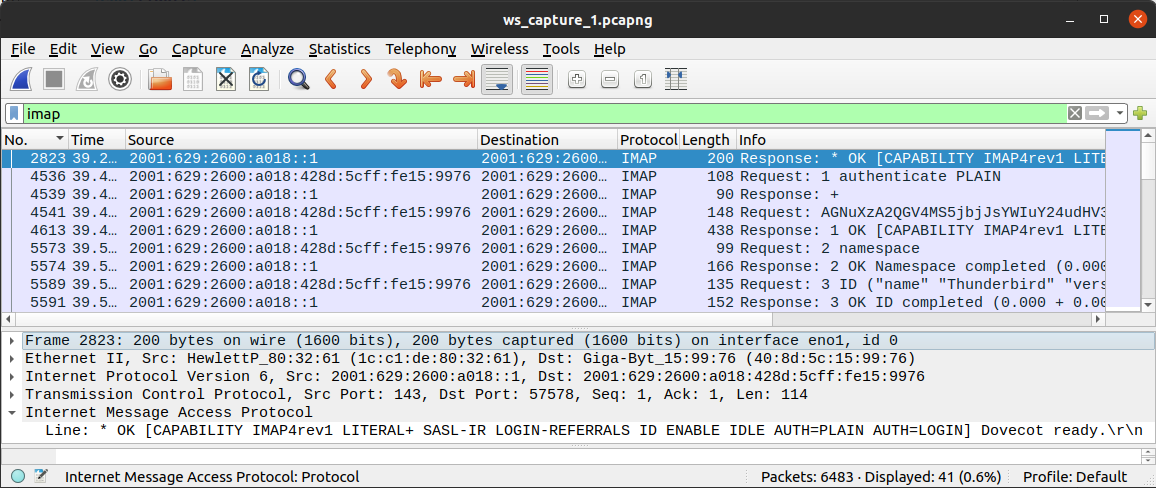
\includegraphics[width=\linewidth]{images/ws1.png} % importing figure
	\caption{Captured IMAP traffic} 
	\label{fig:ws} % labeling to refer it inside the text
\end{figure} 

\subsection{Decoding the messages and find the password} \label{subsec:decode}
As already explained in \cref{sec:task} the client requests to authenticate with plane text and sends its credentials in the fourth exchanged IMAP message to the server. 
Because the credentials are encoded in UTF-8, it is necessary to decode the message string by using the following shell command in the terminal:
\begin{verbatim}
$ base64 -di <<<AGNuXzA2QGV4MS5jbjJsYWIuY24udHV3aWVuLmFjLmF0AFBlZ3Vxb3Rhc2Uy
$ cn_06@ex1.cn2lab.cn.tuwien.ac.atPeguqotase2
\end{verbatim}
In the returned string it is easy to identify the email address followed by the password which is in our case \verb|Peguqotase2|. 

%----------------------------------------------------------------------------------------
%	SECTION 3
%----------------------------------------------------------------------------------------
\section{Conclusion}

This shows how easy it is for attackers to retrieve passwords from plain text email traffic which uses the PLAIN authentication method. Therefore, it is very important to make sure that all connections to the email server are TLS/SSL encrypted. With IMAP this can be done explicitly over port 143, by using the STARTTLS command, or implicitly over port 993 which enforces an encrypted connection.



\printbibliography

%%%%%%%%%%%%%%%%%%%%%%%%%%%%%%%%%%%%%%%%%%%%%%%
\end{document}
